\documentclass[a4paper,12pt]{article}
\usepackage{float} %здесь здесь, только здесь
%%% Работа с русским языком
\usepackage{cmap}					% поиск в PDF
\usepackage{mathtext} 				% русские буквы в формулах
\usepackage[T2A]{fontenc}			% кодировка
\usepackage[utf8]{inputenc}			% кодировка исходного текста
\usepackage[english,russian]{babel}	% локализация и переносы

%%% Дополнительная работа с математикой
\usepackage{amsmath,amsfonts,amssymb,amsthm,mathtools} % AMS
\usepackage{icomma} % "Умная" запятая: $0,2$ --- число, $0, 2$ --- перечисление

%% Номера формул
%\mathtoolsset{showonlyrefs=true} % Показывать номера только у тех формул, на которые есть \eqref{} в тексте.
%\usepackage{leqno} % Нумерация формул слева

%% Свои команды
\DeclareMathOperator{\sgn}{\mathop{sgn}}

%% Перенос знаков в формулах (по Львовскому)
\newcommand*{\hm}[1]{#1\nobreak\discretionary{}
	{\hbox{$\mathsurround=0pt #1$}}{}}

%%% Работа с картинками
\usepackage{graphicx}  % Для вставки рисунков
\graphicspath{{images/}{images2/}}  % папки с картинками
\setlength\fboxsep{3pt} % Отступ рамки \fbox{} от рисунка
\setlength\fboxrule{1pt} % Толщина линий рамки \fbox{}
\usepackage{wrapfig} % Обтекание рисунков текстом

%%% Работа с таблицами
\usepackage{array,tabularx,tabulary,booktabs} % Дополнительная работа с таблицами
\usepackage{longtable}  % Длинные таблицы
\usepackage{multirow} % Слияние строк в таблице

%%% Теоремы
\theoremstyle{plain} % Это стиль по умолчанию, его можно не переопределять.
\newtheorem{theorem}{Теорема}[section]
\newtheorem{proposition}[theorem]{Утверждение}

\theoremstyle{definition} % "Определение"
\newtheorem{corollary}{Следствие}[theorem]
\newtheorem{problem}{Задача}[section]

\theoremstyle{remark} % "Примечание"
\newtheorem*{nonum}{Решение}

%%% Программирование
\usepackage{etoolbox} % логические операторы

%%% Страница
\usepackage{extsizes} % Возможность сделать 14-й шрифт
\usepackage{geometry} % Простой способ задавать поля
\geometry{top=25mm}
\geometry{bottom=35mm}
\geometry{left=35mm}
\geometry{right=20mm}
%

\usepackage{fancyhdr} % Колонтитулы
\pagestyle{fancy}
\renewcommand{\sectionmark}[1]{\markboth{#1}{}}
%\renewcommand{\headrulewidth}{0mm}  % Толщина линейки, отчеркивающей верхний колонтитул
%\lfoot{Нижний левый}
%\rfoot{Нижний правый}
%\rhead{}
%\chead{Верхний в центре}
\lhead{\thepage}
\cfoot{} % По умолчанию здесь номер страницы

\usepackage{setspace} % Интерлиньяж
%\onehalfspacing % Интерлиньяж 1.5
%\doublespacing % Интерлиньяж 2
%\singlespacing % Интерлиньяж 1

\usepackage{lastpage} % Узнать, сколько всего страниц в документе.

\usepackage{soul} % Модификаторы начертания

\usepackage{indentfirst} % Красная строка

\usepackage{soulutf8} % Модификаторы начертания

%\usepackage{hyperref}
%\usepackage[usenames,dvipsnames,svgnames,table,rgb]{xcolor}
%\hypersetup{				% Гиперссылки
%	unicode=true,           % русские буквы в раздела PDF
%	pdftitle={Заголовок},   % Заголовок
%	pdfsubject={Тема},      % Тема
%	pdfcreator={Создатель}, % Создатель
%	pdfproducer={Производитель}, % Производитель
%	pdfkeywords={keyword1} {key2} {key3}, % Ключевые слова
%	colorlinks=true,       	% false: ссылки в рамках; true: цветные ссылки
%	linkcolor=red,          % внутренние ссылки
%	citecolor=green,        % на библиографию
%	filecolor=magenta,      % на файлы
%	urlcolor=cyan           % на URL
%}

%\renewcommand{\familydefault}{\sfdefault} % Начертание шрифта

\usepackage{multicol} % Несколько колонок

\author{\LaTeX{} в Вышке}
\title{3.2 Оформление документа в целом}
\date{\today}

\begin{document} % конец преамбулы, начало документа
	\thispagestyle{empty}
	\begin{center}
		\textit{Федеральное государственное автономное образовательное\\ учреждение высшего образования }
		\vspace{0.5ex}
		
		\textbf{«Московский физико-технический институт\\ (национальный исследовательский университет)»}
	\end{center}
	\vspace{10ex}
	%\begin{flushright}
	%	\noindent
	%	\textit{Фамилия Имя Отчество}
	%	\\
	%	\textit{студент факультета экономики \\(группа 211И)}
	%\end{flushright}
	\begin{center}
		\vspace{13ex}
		\so{\textbf{Лабораторная работа №2.2.1}}
		\vspace{1ex}
		
		по курсу общей физики
		
		
		на тему:
		
		\textbf{\textit{<<Исследование взаимной диффузии газов>>}}
		\vspace{30ex}
		\begin{flushright}
			\noindent
			\textit{Работу выполнил:}
			\\
			\textit{Баринов Леонид \\(группа Б02-827)}
		\end{flushright}
		\vfill
		Долгопрудный \\2019
	\end{center}
	\newpage
	\setcounter{page}{1}
	\section{Аннотация}
	\fancyhead[R]{\nouppercase{\leftmark}}
	В работе будут рассчитаны коэффициенты взаимной диффузии, проведена оценка длины свободного пробега атомов гелия в воздухе $\lambda_{Нe}$ и эффективного сечения столкновений атомов гелия с молекулами воздуха $\sigma_{He-\text{возд}}$.
	\section{Теоретические сведения}
	\subsection{Диффузия}
	Диффузией называют самопроизвольное взаимное проникновение веществ друг в друга, происходящее вследствие хаотичного теплового движения молекул. При перемешивании молекул разного сорта говорят о взаимной (или концентрационной) диффузии.
	\subsection{Закон Фика}
	Диффузия в системе, состоящей из двух компонентов $а$ и $b$ (бинарная смесь), подчиняется закону Фика: плотности потока компонентов 
	$j_{a,b}$ (количество частиц, пересекающих единичную площадку в единицу времени) пропорциональны градиентам их концентраций $\nabla n_{a, b}$, что в одномерном случае можно записать как
\begin{equation*}
\begin{aligned}
j_a = -D\ \frac{\partial  n_a}{\partial  x}, &  & j_b = -D \ \frac{\partial n_b}{\partial x},
\end{aligned}
\end{equation*}
где $D$ — \textit{коэффициент взаимной диффузии компонентов}. Знак «минус» отражает тот факт, что диффузия идёт в направлении выравнивания концентраций. Равновесие достигается при равномерном распределении вещества по объёму сосуда.

В данной работе исследуется взаимная диффузия гелия и воздуха. Давление $P$ и температура $T$ в условиях опыта предполагаются неизменными: 
\[P = (n_{He}+n_\text{в})k_\text{Б} T = const\]
где $n_{He}$ и $n_\text{в}$ — концентрации (объёмные плотности) диффундирующих газов. Поэтому для любых изменений концентраций справедливо $\Delta n_\text{в}$ = -$\Delta n_\text{He}$. Следовательно, достаточно ограничиться описанием диффузии одного из компонентов, например гелия $n_{He}$:
\begin{equation}
j_{He} = -D\ \frac{\partial n_{He}}{\partial x}
\end{equation}

Приведём теоретическую оценку для коэффициента диффузии. В работе концентрация гелия, как правило, мала ($n_{He} \ll n_\text{в}$). Кроме того, атомы гелия
существенно легче молекул, составляющих воздух ($\mu_{He} \ll \mu_{N_2} , \mu_{O_2}$), значит
и их средняя тепловая скорость велика по сравнению с остальными частицами. Поэтому перемешивание газов в работе можно приближенно описывать как диффузию примеси лёгких частиц He на практически стационарном фоне воздуха. Коэффициент диффузии в таком приближении равен
\begin{equation}
D = \frac{1}{3}\lambda \overline{\upsilon} 
\end{equation}
где $\overline{\upsilon}$ -- средняя тепловая скорость частиц примеси, $\lambda$ -- их длина свободного пробега
\begin{equation*}
\begin{aligned}
\overline{\upsilon} = \sqrt{\frac{8RT}{\pi \mu}}, & & & & & & \lambda = \frac{1}{n_0 \sigma}
\end{aligned}
\end{equation*}
$n_0$ -- концентрация рассеивающих центров (фона), $\sigma$ -- сечение столкновения частиц примеси с частицами фона.

В общем случае необходимо учитывать диффузию каждого из компонентов. Более подробное рассмотрение показывает, что для бинарной смеси формула (2) сохраняется, если под $\lambda$ понимать величину 
\begin{equation*}
\begin{aligned}
\lambda = \frac{1}{n\sigma}, & & & & & n = n_{He}+n_\text{в} = \frac{P}{k_\text{Б}T}
\end{aligned}
\end{equation*}
под $\overline{\upsilon}$
понимать среднюю относительную скорость частиц разных сортов.

Таким образом, теория предсказывает, что коэффициент диффузии бинарной смеси обратно пропорционален давлению в системе 
\[D \propto \frac{1}{P}\]
и не зависит от пропорций компонентов, что и будет проверено в эксперименте

\subsection{Схема эксперимента}

Для исследования взаимной диффузии газов и измерения коэффициента взаимной диффузии $D$ используется два сосуда объёмами $V_1$ и $V_2$ ($V_1\approx V_2 \equiv V$), соединенные трубкой длины $L$ и сечения $S$ (Рис. 1).
\begin{wrapfigure}{r}{0.2\linewidth}
	\includegraphics[width=\linewidth]{1}
	\caption{}
\end{wrapfigure}
 Предполагается, что сосуды заполнены смесью двух газов при одинаковом давлении, но с различной концентрацией компонентов. Вследствие взаимной диффузии, проходящей в соединительной трубке, концентрации компонентов в сосудах с течением времени выравниваются.
 
 \noindent Применим закон Фика в трубке, получим
 \[j = -D\ \frac{\partial n}{\partial x} = const\]
Следовательно, распределение концентрации в трубке $n(x)$ — линейная функция:
\begin{equation}
n(x) = \frac{\Delta n}{L}x
\end{equation}
и плотность потока частиц всюду постоянна и равна
\begin{equation}
j = -D \frac{\Delta n}{L}
\end{equation}
где $\Delta n = n_2- n_1$ -- разность концентраций гелия на концах трубки.

Полное число частиц примеси в сосудах равно соответственно $N_1 = n_1V$ и $N_2 = n_2 V$. Произведение плотности потока (4) на площадь сечения трубки $S$ даёт количество частиц, пересекающих в единицу времени любое поперечное сечение трубки. Поэтому
\begin{equation}
\begin{aligned}
\frac{dN_1}{dt} = jS, & & & \frac{dN_2}{dt} = -jS.
\end{aligned}
\end{equation}
Выразим отсюда скорость изменения $\Delta n$. Вычитая из второго равенства первое и деля результат на объём сосуда $V$, с учетом (4) получим
\begin{equation}
\frac{d(\Delta n)}{dt} = - \frac{\Delta n}{\tau}
\end{equation}
где введено обозначение
\begin{equation}
\tau = \frac{1}{D}\frac{VL}{2S}
\end{equation}
Интегрируя (6), получаем, что разность концентраций будет убывать по экспоненциальному закону
\begin{equation}
\Delta n = \Delta n_0 e^{-t/\tau}
\end{equation}
где $\Delta n_0$ — разность концентраций примеси в сосудах в начальный момент времени. Видно, что величина $\tau$ есть \textit{характерное время} выравнивания концентраций между сосудами. Оно определяется геометрическими размерами установки и коэффициентом диффузии.

Отметим, что для применимости квазистационарного приближения необходимо убедиться, что время процесса $\tau$ много больше характерного времени диффузии отдельной частицы вдоль трубки $L$, которое согласно
закону Эйнштейна-Смолуховского по порядку величины равно
\begin{equation}
\tau_{\text{диф}} \sim \frac{L^2}{2 D}
\end{equation}
\section{Оборудование}
\subsection{Методика измерений}
Для измерения разности концентраций в установке применяются датчики теплопроводности. При этом используется тот факт, что теплопроводность $\kappa$ смеси зависит от её состава. В общем случае зависимость $\kappa (n)$ довольно сложна, однако при малой разности $\Delta n$ концентраций в сосудах можно ожидать, что разность теплопроводностей будет изменяться прямо пропорционально $\Delta n$:
\[\Delta \kappa = \kappa(n_2) - \kappa(n_1) \approx const \cdot \Delta n\]
\subsection{Датчики теплопроводности}
Сами датчики теплопроводности устроены следующим образом. Тонкая платиновая проволочка, протянутая вдоль оси стеклянного цилиндра, нагревается током. Внутренняя полость датчика сообщается с объёмом камеры через отверстия, размеры которых таковы, что скорость диффузии из объёма сосуда в полость датчика значительно больше скорости диффузии из одного объёма в другой. Таким образом, состав газа в датчике практически совпадает с составом газа в объёме. Тепло от проволочки к стенке цилиндра передаётся главным образом за счёт теплопроводности газа, находящегося внутри цилиндра. При заданной мощности нагревания приращение температуры проволочки и, следовательно, приращение её сопротивления пропорциональны теплопроводности газа
\subsection{Мостовая схема}
\begin{wrapfigure}{r}{0.3\linewidth}
	\includegraphics[width=\linewidth]{5}
	\caption{Мостовая схема}
\end{wrapfigure}
Для измерения сопротивлений используется мостовая схема, позволяющая определять разность показаний датчиков с высокой точностью. Мост балансируется при заполнении сосудов (и датчиков) одной и той же смесью. При заполнении сосудов смесями различного состава возникает «разбаланс» моста. При незначительном различии в составах смесей показания вольтметра, подсоединённого к диагонали моста, будут пропорциональны разности концентраций примеси: $U \propto \Delta\kappa \propto\Delta n$. В процессе диффузии разность концентраций убывает по закону (8), и значит по тому же закону изменяется напряжение:
\begin{equation}
U = U_0 e^{-t/\tau}
\end{equation}
де $U_0$ — показание гальванометра в начальный момент времени. Измеряя экспериментально зависимость $U(t)$, можно получить характерное время процесса $\tau$, откуда по формуле (7) определить коэффициент диффузии $D$.

Датчики теплопроводности $\text{Д}_1$ и $\text{Д}_2$, расположенные в сосудах $V_1$ и $V_2$ соответственно, включены в мостовую электрическую схему согласно рис. 2. В одну из диагоналей моста включён высокочувствительный вольтметр (гальванометр) $\text{Г}$, к другой подключается источник небольшого постоянного напряжения. Сопротивления проволок датчиков составляют одно из плеч моста. Второе плечо составляют переменные сопротивления $R_1$, $R_2$ и $R$, служащие для установки показаний вольтметра $\text{Г}$ на нуль (балансировка моста). Сопротивления $R_1$ и $R_2$ спарены (их подвижные контакты находятся на общей оси) и изменяются одновременно при повороте ручки грубой регулировки. Точная балансировка выполняется потенциометром $R$. Балансировку необходимо проводить перед каждым экспериментом заново: при этом установка заполняется чистым газом (воздухом без гелия) при давлении, близком «рабочему» (при котором затем будут проводится измерения).
\subsection{Эксперементальная установка}
\begin{figure}[h]
	\begin{center}
		\begin{minipage}[h]{0.25\linewidth}
			\includegraphics[width=1\linewidth]{2}
		\end{minipage}
		\begin{minipage}[h]{0.3\linewidth}
			\includegraphics[width=1\linewidth]{3}
		\end{minipage}
	\end{center}
\caption{Схема измерительной части установки с конструкцией системы откачки и напуска }
\end{figure}
Измерительная часть установки состоит из двух сосудов $V_1$ и $V_2$, размещённых вертикально. Краны $\text{К}_1$ и $\text{К}_2$ служат для управления откачкой и подачей воздуха/гелия в сосуды. Диффузия осуществляется через тонкую короткую трубку, соединяющую сосуды, оснащённую краном $\text{К3}$. К соединительным трубкам подключен манометр M, измеряющий разность давлений между соединительными трубками и атмосферой, и позволяющий измерять давления в разных частях системы (в зависимости от положения кранов).

\begin{wrapfigure}{r}{0.2\linewidth}
	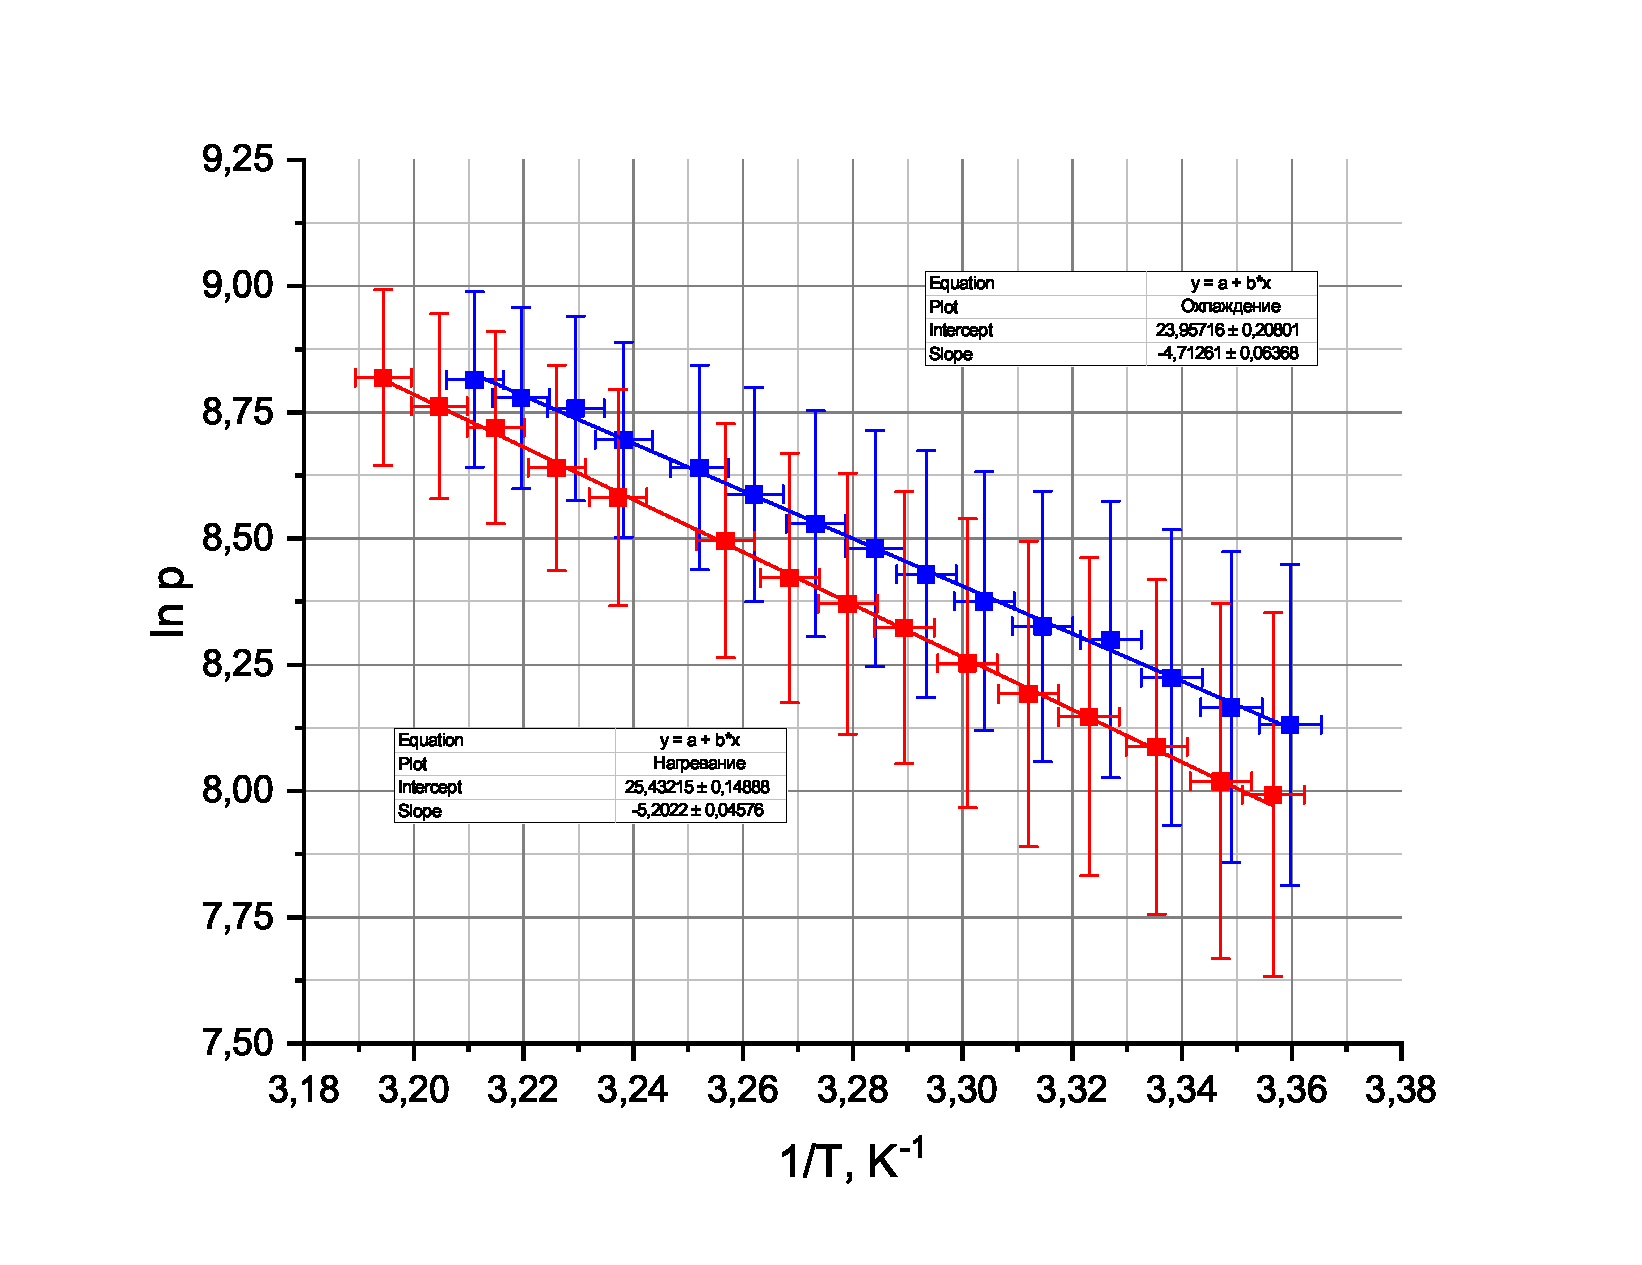
\includegraphics[width=\linewidth]{4}
	\caption{Двухходовый кран}
\end{wrapfigure}

Гелий содержится в баллоне  под давлением, превышающим атмосферное. Для предотвращения избыточного расхода гелия и его неконтролируемого проникания в установку предусмотрен металлический кран $К_7$, отделяющий её от баллона с гелием. Его открывают только на время непосредственного заполнения установки гелием, остальное время он должен быть закрыт. Для подачи малых порций гелия предусмотрен двухходовый кран с дозатором (рис. 4). При повороте рычажка $\text{Р}$ в положение $I$ гелий в небольшом количестве поступает в дозатор (если открыт $\text{K}_7$), а при повороте $\text{Р}$ в положение $II$ порция из дозатора поступает в установку.

\renewcommand{\arraystretch}{1.1}
\section{Результаты измерений и обработка результатов}
Для разных давлений  снимем зависимость напряжения от времени. Результаты занесем в таблицу 1.
\begin{longtable}{|c|c|c|c|c|c|c|c|}
	\hline
	\multicolumn{2}{|c|}{$P_1 = 40\ \text{торр}$} & \multicolumn{2}{|c|}{$P_2 = 100 \ \text{торр}$} & \multicolumn{2}{|c|}{$P_3 = 150\ \text{торр}$} & \multicolumn{2}{|c|}{$P_4 = 200\ \text{торр}$} \\ \hline
	\rule{0cm}{3ex}
		$t, \text{c}$ &  $\ln \frac{U}{U_0}$  & $t, \text{c}$ & $\ln \frac{U}{U_0}$ & $t, \text{c}$  & $\ln \frac{U}{U_0}$   & $t, \text{c}$  & $\ln \frac{U}{U_0}$   \\ [1ex]\hline
	\endfirsthead
	\hline
	\multicolumn{2}{|c|}{$P_1 = 40\ \text{торр}$} & \multicolumn{2}{|c|}{$P_2 = 100 \ \text{торр}$} & \multicolumn{2}{|c|}{$P_3 = 150\ \text{торр}$} & \multicolumn{2}{|c|}{$P_4 = 200\ \text{торр}$} \\ \hline
		\rule{0cm}{3ex}
		$t, \text{c}$ &  $\ln \frac{U}{U_0}$  & $t, \text{c}$ & $\ln \frac{U}{U_0}$ & $t, \text{c}$  & $\ln \frac{U}{U_0}$   & $t, \text{c}$  & $\ln \frac{U}{U_0}$   \\ [1ex]\hline
	\endhead
	\hline
	\endfoot
	\endlastfoot
0,00   & 0,000    & 0,00   & 0,000    & 0,00   & 0,000    & 0,00   & 0,000    \\ \hline
11,85  & 0,033    & 10,48  & 0,016    & 10,62  & 0,008    & 10,53  & 0,004    \\ \hline
23,71  & 0,067    & 20,96  & 0,028    & 21,24  & 0,013    & 21,05  & 0,004    \\ \hline
35,56  & 0,098    & 31,44  & 0,040    & 31,85  & 0,020    & 31,58  & 0,008    \\ \hline
47,41  & 0,134    & 41,92  & 0,052    & 42,47  & 0,028    & 42,11  & 0,012    \\ \hline
59,27  & 0,171    & 52,40  & 0,069    & 53,09  & 0,036    & 52,63  & 0,012    \\ \hline
71,12  & 0,211    & 62,88  & 0,082    & 63,71  & 0,040    & 63,16  & 0,008    \\ \hline
82,97  & 0,248    & 73,36  & 0,095    & 74,32  & 0,048    & 73,68  & 0,008    \\ \hline
94,83  & 0,284    & 83,84  & 0,106    & 84,94  & 0,052    & 84,21  & 0,008    \\ \hline
106,68 & 0,326    & 94,32  & 0,121    & 95,56  & 0,051    & 94,74  & 0,012    \\ \hline
118,54 & 0,369    & 104,81 & 0,137    & 106,18 & 0,048    & 105,26 & 0,016    \\ \hline
130,39 & 0,411    & 115,29 & 0,148    & 116,80 & 0,056    & 115,79 & 0,020    \\ \hline
142,24 & 0,454    & 125,77 & 0,161    & 127,41 & 0,065    & 126,32 & 0,020    \\ \hline
154,10 & 0,491    & 136,25 & 0,175    & 138,03 & 0,073    & 136,84 & 0,024    \\ \hline
165,00 & 0,531    & 146,73 & 0,189    & 148,65 & 0,086    & 147,37 & 0,028    \\ \hline
177,80 & 0,571    & 157,21 & 0,199    & 159,27 & 0,099    & 157,89 & 0,032    \\ \hline
189,66 & 0,614    & 167,69 & 0,209    & 169,89 & 0,103    & 168,42 & 0,036    \\ \hline
201,51 & 0,654    & 178,17 & 0,223    & 180,50 & 0,108    & 178,95 & 0,040    \\ \hline
213,36 & 0,695    & 188,65 & 0,234    & 191,12 & 0,109    & 189,47 & 0,048    \\ \hline
225,22 & 0,729    & 199,13 & 0,248    & 201,74 & 0,108    & 200,00 & 0,052    \\ \hline
237,07 & 0,771    & 209,61 & 0,259    & 212,36 & 0,112    & 210,00 & 0,056    \\ \hline
248,92 & 0,809    & 220,09 & 0,273    & 222,97 & 0,116    & 221,00 & 0,065    \\ \hline
260,78 & 0,841    & 230,57 & 0,284    & 233,59 & 0,121    & 231,00 & 0,069    \\ \hline
272,63 & 0,887    & 241,05 & 0,279    & 244,21 & 0,112    & 242,11 & 0,073    \\ \hline
		\caption{Зависимость логарифма  $\ln U/U_0$ от времени $t$ при различных давлениях}
\end{longtable}
\renewcommand{\arraystretch}{1}
По данным в Таблице 1 построим график зависимости логарифма отношения $\ln U/U_0$ от времени $t$ для различных давлений. (Рис. 5). По наклону прямых рассчитаем характерное время выравнивания концентраций $\tau$ между сосудами по формуле (10). Далее рассчитаем коэффициент взаимной диффузии $D$ по формуле (7). Результаты занесем в Таблицу 2.

\begin{table}[H]
	\begin{center}
	\begin{tabular}{|c|c|c|c|c|}
		\hline
		$P, \text{торр}$   & $\tau, \text{с}$       & $\Delta \tau, \text{с}$      & $D, \text{см}^2/\text{с}$     & $\Delta D, \text{см}^2/\text{с}$    \\ \hline
		40  & 311,53  & 1,46   & 10,59 & 1,00 \\ \hline
		100 & 806,45  & 5,14   & 4,09  & 0,39 \\ \hline
		150 & 1855,29 & 36,83  & 1,78  & 0,17 \\ \hline
		200 & 4132,23 & 196,37 & 0,80  & 0,08 \\ \hline
	\end{tabular}
\caption{Характерное время выравнивания концентраций $\tau$ и коэффициент взаимной диффузии $D$ для различных давлений $P$}
\end{center}
\end{table}

\begin{figure}[H]
	\begin{center}
		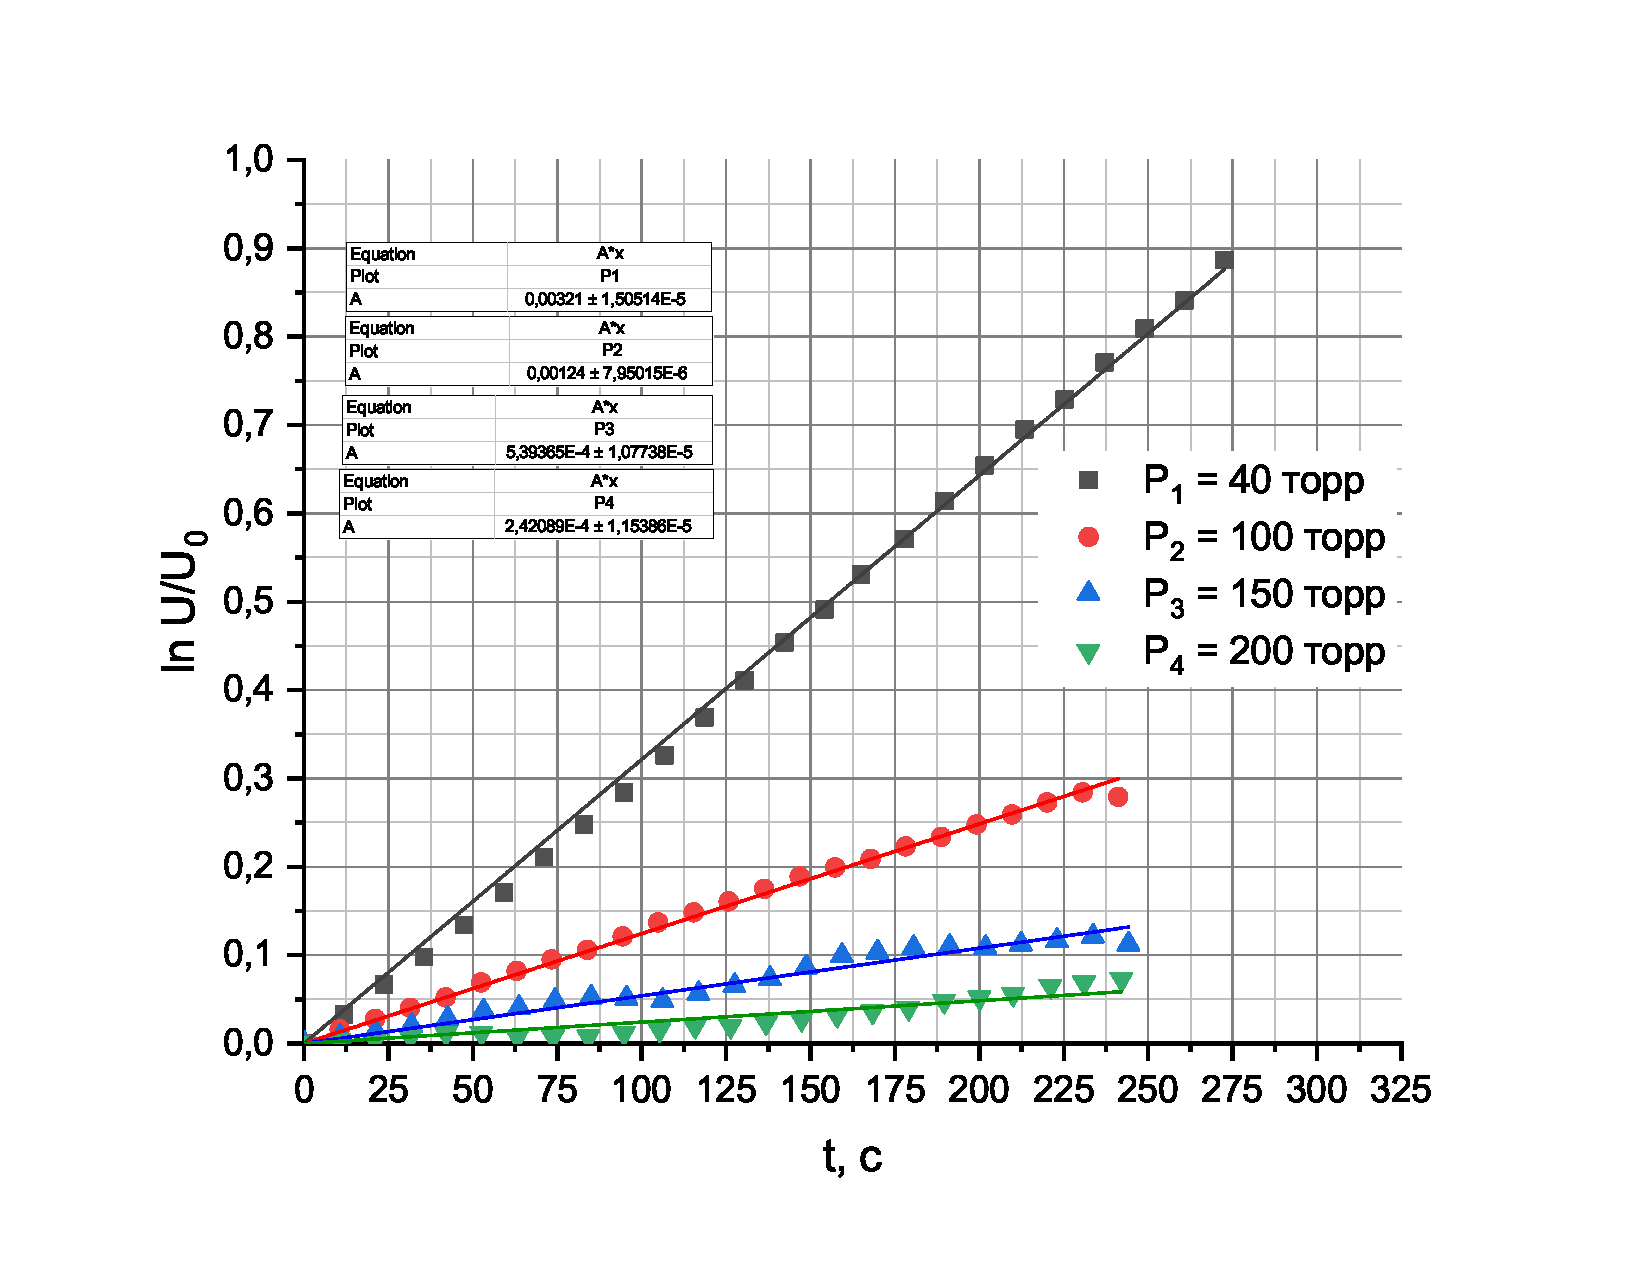
\includegraphics[width=\linewidth]{6}
		\caption{ график зависимости логарифма $\ln U/U_0$ от времени $t$ для различных давлений $P$}
	\end{center}
\end{figure}
Построим график зависимости коэффициента диффузии от обратного давления по результатам в Таблице 2. (Рис. 6) Экстраполируя график к атмосферному давлению, оценим соответствующий коэффициент диффузии.
\[D_\text{атм} = (0,71\pm0,07)\ \text{см}^2/\text{с}\]

Проверим утверждения о независимости коэффициента взаимной диффузии от пропорций компонентов. Проведем измерение коэффициента диффузии примеси воздуха в гелии. Результаты занесем в Таблицу 3.

Построим график по данным из Таблицы 3 и сравним его с графиком, когда исследовалась примесь гелия в воздухе при $P = 40\ \text{торр}$ (Рис. 7). По графику вычислим значение коэффициента взаимной диффузии.
\[ D_{\text{возд} - He} = (12,3\pm1,2) \text{см}^2/\text{с}  \]
Оценим длину свободного пробега атомов гелия в воздухе, используя \\ формулу (2)
\[\lambda \approx 10^{-7}\ \text{м}\]
\newpage
Произведем оценку эффективного сечения столкновений атомов гелия с молекулами воздуха.

\[\sigma_{He - \text{возд}} \approx  10^{-19}\ \text{м}^2\]
\begin{figure}[H]
	\begin{center}
		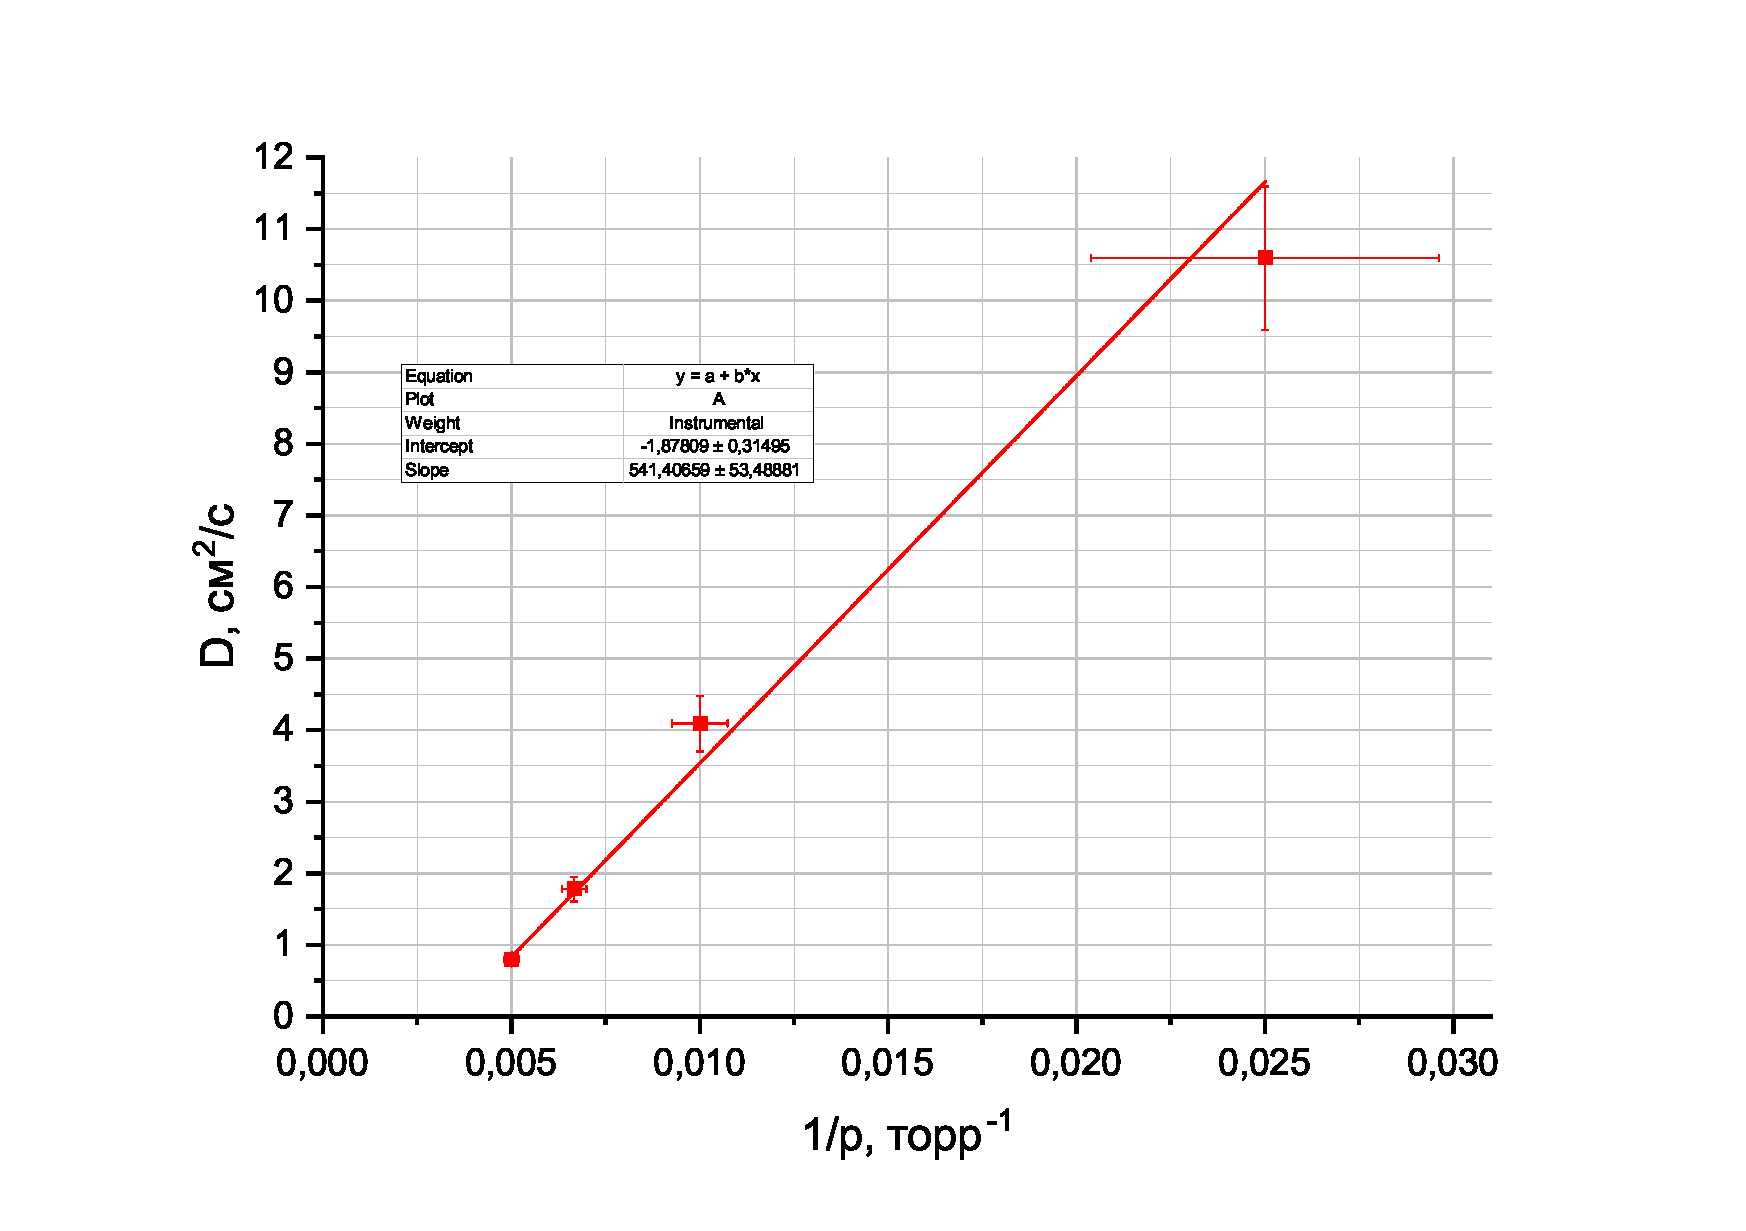
\includegraphics[width=\linewidth]{7}
		\caption{Зависимость коэффициента взаимной диффузии $D$ от величины, обратной к давлению $1/P$}
	\end{center}
\end{figure}



\begin{table}[H]
	\begin{center}

	\begin{tabular}{|c|c|c|c|c|c|c|c|c|}
		\hline
		$t, \text{с}$ & 0,00  & 9,61  & 19,22 & 28,83 & 38,44 & 48,05 & 57,67 & 67,28   \\ \hline
		\rule{0cm}{3ex}
		$\ln \frac{U}{U_0}$& 0,000 & 0,053 & 0,100 & 0,179 & 0,218 & 0,256 & 0,288 & 0,320    \\ [1ex]\hline \hline
		$t, \text{с}$& 76,89 & 86,50 & 96,11 & 105,72 & 115,33 & 124,94 & 134,55 & 144,16   \\ \hline
		\rule{0cm}{3ex}
		$\ln \frac{U}{U_0}$& 0,348  & 0,376 & 0,400 & 0,426  & 0,454  & 0,483  & 0,510  & 0,530    \\[1ex] \hline \hline
		$t, \text{с}$ & 153,78 & 163,39 &173,00 & 182,61 & 192,22 & 201,83 & 211,44 & 221,05 \\ \hline
		\rule{0cm}{3ex}
		$\ln \frac{U}{U_0}$& 0,558  & 0,593 &0,614  & 0,647  & 0,674  & 0,705  & 0,769  & 0,805  \\[1ex]  \hline
	\end{tabular}
\end{center}
\caption{Зависимость логарифма $\ln U/U_0$ от времени $t$ при исследовании примеси воздуха в гелии (суммарное давление $P = 40\ \text{торр}$)}
\end{table}

\begin{figure}[H]
	\begin{center}
		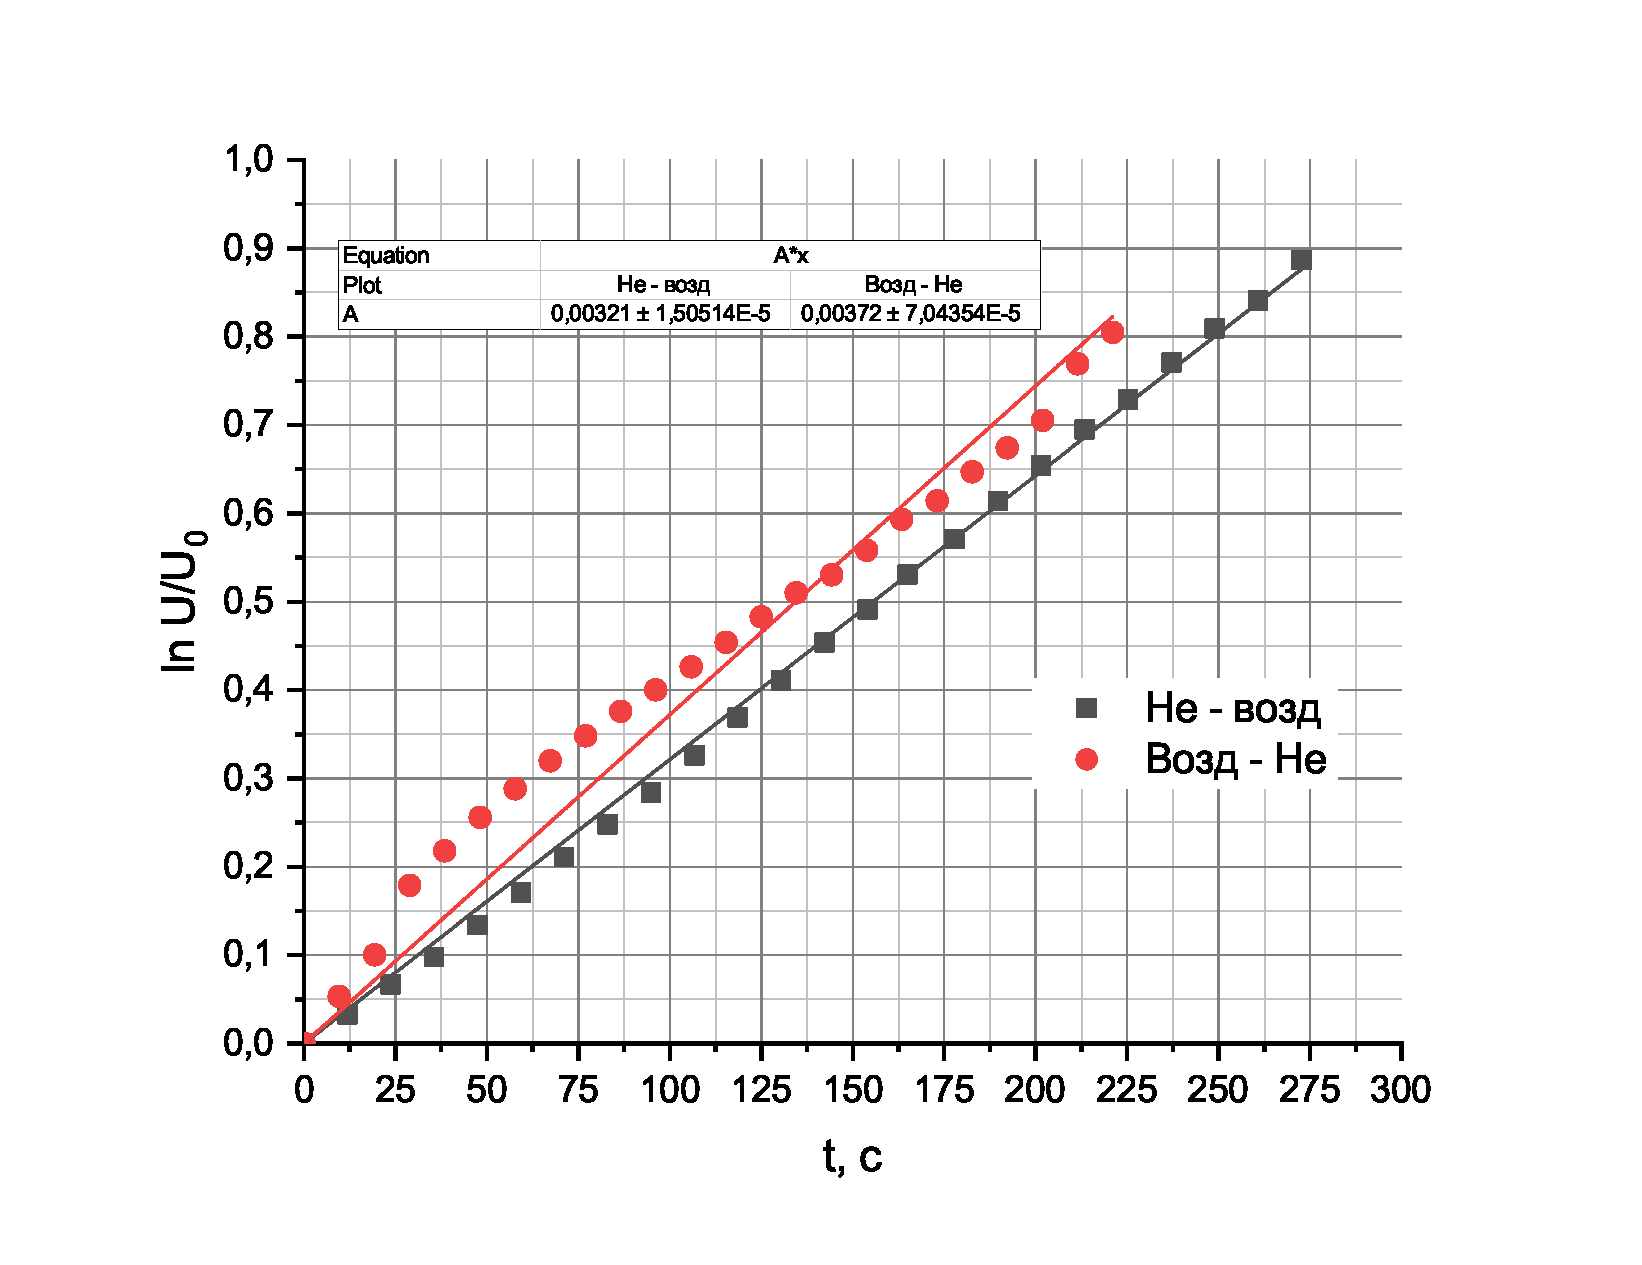
\includegraphics[width=\linewidth]{8}
	\end{center}
\caption{Зависимость $\ln U/U_0$ от $t, \text{с}$ при исследовании примеси $He$ в воздухе и примеси воздуха в $He$ }
\end{figure}
\section{Обсуждение результатов и выводы}
В работе были проведены измерения характерного времени выравнивания концентраций $\tau$ и коэффициента взаимной диффузии воздуха и гелия $D$. \\(Таблица 2)

Были проведены вычисления коэффициента диффузии при атмосферном давлении путем экстраполирования графика зависимости коэффициента взаимной диффузии $D$ от величины, обратной к давлению $1/P$ (Рис. 6)
\[D_\text{атм} = (0,71\pm0,07)\ \text{см}^2/\text{с}\] 
Значение с учетом погрешности попадает в табличное значение:
\[D_\text{атм}^\text{т} = 0,73\ \text{см}^2/\text{с} \]

Также проведена оценка длины свободного пробега атомов гелия в воздухе $\lambda$ и эффективного сечения столкновений атомов гелия с молекулами воздуха $\sigma_{He - \text{возд}}$ по порядку величины.
\[\lambda \approx 10^{-7}\ \text{м}\]
\[\sigma_{He - \text{возд}} \approx  10^{-19}\ \text{м}^2\]

Было проверено утверждения о независимости коэффициента взаимной диффузии от пропорций компонентов. (Рис 7)
\[ D_{He - \text{возд}} = (10,6\pm1,0)\ \text{см}^2/\text{с}  \]
\[ D_{\text{возд} - He} = (12,3\pm1,2)\ \text{см}^2/\text{с}  \]
C учетом погрешностей можно считать, что
\[D_{He - \text{возд}} \approx D_{\text{возд} - He}\]
Следовательно, утверждение верно.
\end{document}